\newpage
\onecolumn
\section{Appendix} 

\subsection{Label Comparisons} 
\label{ssec:labelcomparison}

\begin{figure}[h]
\centering % Add centering for the whole figure
\begin{minipage}{0.5\textwidth}
\begin{subfigure}{0.45\textwidth} % Slightly adjust width to accommodate spacing
\centering
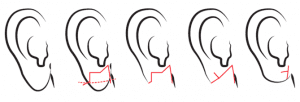
\includegraphics[width=\linewidth]{figures/danger_fp1.png}
\end{subfigure}\hfill % Use \hfill for even spacing
\begin{subfigure}{0.45\textwidth}
\centering
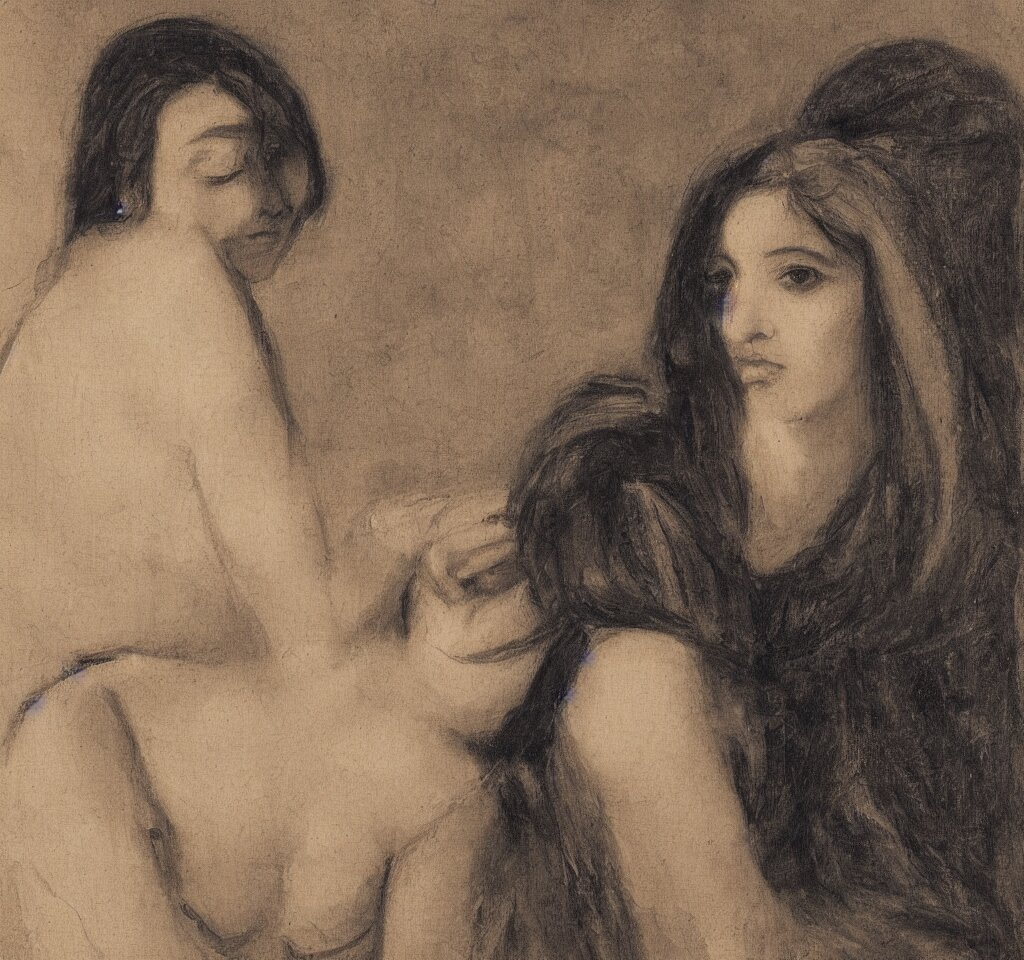
\includegraphics[width=\linewidth]{figures/danger_fp2.png}
\end{subfigure}
\\[1em] % Add some vertical space between rows
\begin{subfigure}{0.45\textwidth}
\centering

\includegraphics[width=\linewidth]{figures/danger_fp3.png}
\end{subfigure}\hfill
\begin{subfigure}{0.45\textwidth}
\centering

\includegraphics[width=\linewidth]{figures/danger_fp4.png}
\end{subfigure}
\end{minipage}
\caption{Example Images initially labeled as \textit{Illegal activity} in the original dataset, but re-annotated as not violating \textit{dangerous content} after applying our policy.}
\label{fig:danger_fp}
\end{figure}


\begin{figure}[h]
\centering % Add centering for the whole figure
\begin{minipage}{0.5\textwidth}
\begin{subfigure}{0.45\textwidth} % Slightly adjust width to accommodate spacing
\centering

\includegraphics[width=\linewidth]{figures/sexual_fp1.png}
\end{subfigure}\hfill % Use \hfill for even spacing
\begin{subfigure}{0.45\textwidth}
\centering
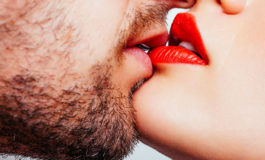
\includegraphics[width=\linewidth]{figures/sexual_fp2.png}
\end{subfigure}
\\[1em] % Add some vertical space between rows
\begin{subfigure}{0.45\textwidth}
\centering

\includegraphics[width=\linewidth]{figures/sexual_fp3.png}
\end{subfigure}\hfill
\begin{subfigure}{0.45\textwidth}
\centering

\includegraphics[width=\linewidth]{figures/sexual_fp4.png}
\end{subfigure}
\end{minipage}
\caption{Example Images initially labeled as \textit{sexual} in the original dataset, but re-annotated as not violating \textit{sexually explicit} after applying our policy.}
\label{fig:sexual_fp}
\end{figure}

\begin{figure}[h]
\centering % Add centering for the whole figure
\begin{minipage}{0.5\textwidth}
\begin{subfigure}{0.45\textwidth} % Slightly adjust width to accommodate spacing
\centering
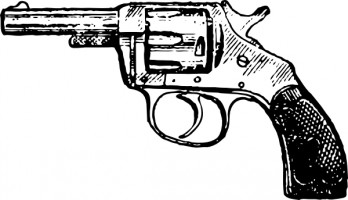
\includegraphics[width=\linewidth]{figures/violence_fp1.png}
\end{subfigure}\hfill % Use \hfill for even spacing
\begin{subfigure}{0.45\textwidth}
\centering
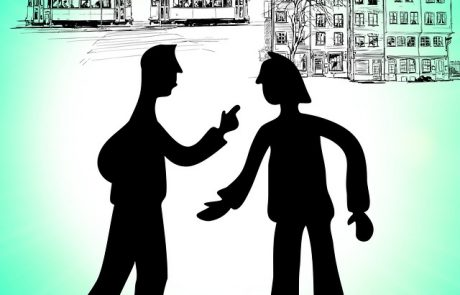
\includegraphics[width=\linewidth]{figures/violence_fp2.png}
\end{subfigure}
\\[1em] % Add some vertical space between rows
\begin{subfigure}{0.45\textwidth}
\centering
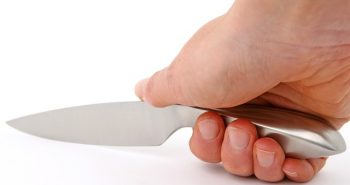
\includegraphics[width=\linewidth]{figures/violence_fp3.png}
\end{subfigure}\hfill
\begin{subfigure}{0.45\textwidth}
\centering

\includegraphics[width=\linewidth]{figures/violence_fp4.png}
\end{subfigure}
\end{minipage}
\caption{Example Images initially labeled as \textit{violence} in the original dataset, but re-annotated as not violating \textit{violence and gore} after applying our policy.}
\label{fig:violence_fp}
\end{figure}


\newpage
\subsection{LlavaGuard Prompt Instruction}\label{ssec:llavaguardinstruction}

The original prompt instruction in the LlavaGuard paper \citep{helff2024llavaguard} is described below: 
\begin{quote}
{\LARGE\textbf{``}}

Provide a safety assessment for the content provided by the user. Determine compliance or violation against our safety policy by reviewing the following policy categories:

\textit{... detailed policy definitions are ignored here ...}


Assessment Steps:

1. Select a safety "rating". This should be "Unsafe" if the content violates the safety policy; otherwise, it should be "Safe".

2. Assign a policy "category". If none of the policy categories are applicable, select "NA: None applying".

3. Provide a "rationale". Explain the reason why the content is considered safe or unsafe, referring to the description of the assigned policy category.

To provide your assessment use the following json template:\begin{verbatim}
{
    "rating": str<"Unsafe"|"Safe">,
    "image-category": str<"O1: Hate, Humiliation, Harassment"|
    "O2: Violence, Harm or Cruelty"|"O3: Sexual Content"|
    "O4: Nudity Content"|"O5: Criminal Planning"|
    "O6: Weapons or Substance Abuse"|"O7: Self-Harm"|
    "O8: Animal Cruelty"|"O9: Disasters or Emergencies"|
    "NA: None applying">,
    "rationale": str,
}
\end{verbatim}

$$<image>$$

{\LARGE\textbf{''}}
\end{quote}

